\newcommand{\School}{Academic Institution}
\newcommand{\Class}{Class Title}
\newcommand{\Assignment}{Assignment Title}
\newcommand{\Name}{Your \textsc{Name}}
\newcommand{\Professor}{Professor's \textsc{Name}}
\newcommand{\Duedate}{\today}

\documentclass[11pt]{article}
\usepackage{geometry}
\geometry{letterpaper}

\usepackage{amssymb,amsmath,cancel}
\usepackage{caption, subcaption}
\usepackage{setspace}
\usepackage{fullpage}
\usepackage{lipsum}
\usepackage{tikz}	
\usetikzlibrary{decorations.pathreplacing, calc}
\usetikzlibrary{snakes,shapes,decorations.text}

\let\underdot=\d
\renewcommand{\d}[2]{\frac{d #1}{d #2}}
\newcommand{\dd}[2]{\frac{d^2 #1}{d #2^2}}
\newcommand{\pd}[2]{\frac{\partial #1}{\partial #2}}
\newcommand{\pdd}[2]{\frac{\partial^2 #1}{\partial #2^2}}
\newcommand{\degrees}{\ensuremath{^\circ}}

\begin{document}
  
  \begin{titlepage}
    \newcommand{\HRule}{\rule{\linewidth}{0.5mm}}
    \center
    \textsc{\LARGE \School}\\[1.5cm]
    \textsc{\Large \Class}\\[0.3cm]
    \HRule \\[0.4cm]
    { \huge \bfseries \Assignment}\\[0.1cm] 
    \HRule \\[1.5cm]
    \begin{minipage}{0.4\textwidth}
      \begin{flushleft} \large
        \emph{Author:}\\
        \Name
        \end{flushleft}
        \end{minipage}
        ~
        \begin{minipage}{0.4\textwidth}
        \begin{flushright} \large
        \emph{Course Instructor:} \\
        \Professor \\
      \end{flushright}
    \end{minipage}
      \\[1cm]
    {\large \Duedate}\\[3cm]
    \vfill
  \end{titlepage}

  \newpage 
  \begin{abstract}
    \lipsum[1-3]
  \end{abstract}

  \newpage 
  \tableofcontents
  \listoffigures

  \newpage
  \section{Section}
  Cras nibh. Morbi vel justo vitae lacus tincidunt ultrices. Lorem ipsum dolor sit amet, consectetuer adipiscing elit.
  \subsection{Derivation}
  Fusce mauris. Vestibulum luctus nibh at lectus. Sed bibendum, nulla a faucibus semper, leo velit ultricies tellus, ac venenatis arcu wisi vel nisl. 
  Quisque ullamcorper placerat ipsum. $x^2$. Et, $y = 10\degrees$.
  Praesent enim elit, rutrum at, molestie non, nonummy vel, nisl. Ut lectus eros, malesuada sit amet, fermentum eu, sodales cursus, magna.
  $$ x^2 + y^2 = z^2 $$
  Donec eu purus. Quisque vehicula, urna sed ultricies auctor, pede lorem egestas dui, et convallis elit erat sed nulla. Donec luctus. Curabitur et nunc.
  
  \begin{align*}
    z^2 &= x^2 + y^2 \\
    z &= \sqrt{x^2 + y^2} \\
    \dot z = \d{z}{t} &= \d{\sqrt{x^2+y^2}}{t} = \d{}{t}\sqrt{x^2+y^2}
  \end{align*}
  
  See Figure~\ref{named_schematic} on pp.~\pageref{named_schematic}.
  
  \begin{figure}[p]
    \begin{center}
      
      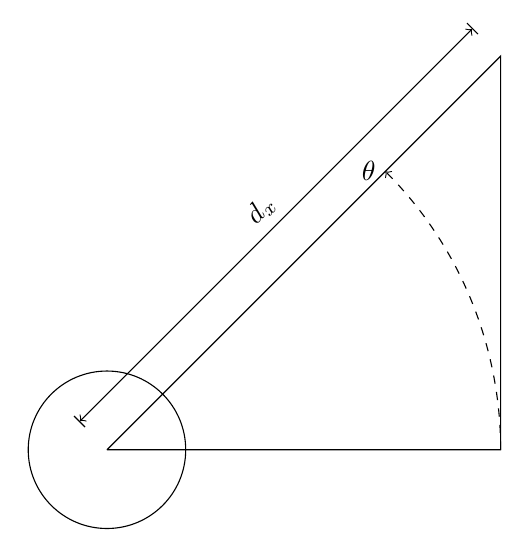
\begin{tikzpicture}
        \coordinate(O) at (0,0);
        \coordinate(A) at (5,0);
        \coordinate(B) at (5,5);
        \draw (O)--(A)--(B)--(O);
        \draw (O) circle [radius=1];
        \draw [|<->|] ($(O)+(135:0.5)$) -- ($(B)+(135:0.5)$) node[midway, above, sloped] {$d_x$};
        \draw [->, dashed] (A) arc ( 0 : 45 : 5) node[anchor=east] {$\theta$};
      \end{tikzpicture}

    \end{center}
    \caption{Schematic with Title}
    \label{named_schematic}
  \end{figure}
\end{document}
